% !Mode:: "TeX:UTF-8"
% VL 5, gebaut aus part-lernen/07-loss-funktionen-maximum-likelihood.md
% und part-lernen/08-gradientenabstieg.md
% (Dialogmuster und Zeiten: transcripts/vl05-sgd-2025/notiz.md).
% !Mode:: "TeX:UTF-8"
\newcommand{\thepage}{} % to silence a hyperref warning about pdfpagelabels
\RequirePackage[]{silence}
\WarningsOff[hyperref]
\PassOptionsToPackage{log-declarations=false}{xparse}
%\RequirePackage[l2tabu, orthodox]{nag}
\RequirePackage{luatex85} % to make \pdf...= commands work with LuaTeX
\documentclass[aspectratio=169,t]{beamer}
\usepackage{ifthen}
\usepackage[T1]{fontenc}
\usepackage{iftex}
\ifLuaTeX
 \usepackage{fontspec}
 \setmainfont[Ligatures=TeX]{Source Sans Pro}
\else
 \usepackage[utf8]{inputenc}
\fi
\usepackage{german}
\usepackage{newunicodechar}
\newunicodechar{€}{\texteuro}
\newunicodechar{ß}{\ss}
\renewcommand{\SS}{\iffontchar\font"1E9E \symbol{"1E9E}\else SS\fi}
\usepackage{ellipsis}
\usepackage{microtype}
\usepackage{listings}
\usepackage{sourcecodepro}
\lstset{language=Python, basicstyle=\ttfamily}
\usepackage{amsfonts}
\usepackage{amssymb}
\usepackage{amsthm}
\usepackage{fancyhdr}
\usepackage{graphicx}

\newtheorem{proposition}[theorem]{Proposition}

\DeclareMathOperator*{\argmax}{argmax}
\DeclareMathOperator{\supp}{supp}
\newcommand{\E}{\ensuremath{\mathbb{E}}}
\newcommand{\V}{\ensuremath{\mathbb{V}}}

\setbeamercolor{emph}{fg=purple}
\renewcommand<>{\emph}[1]{%
  {\usebeamercolor[fg]{emph}\only#2{\itshape}#1}%
}



\hypersetup{draft=false,colorlinks=false,pdfpagemode=UseOutlines,plainpages=false,
            breaklinks=true,bookmarksnumbered=true,pdfborder=0 0 0,
            pdftitle={Einführung in Deep Learning WiSe 2026/27 HHU},
            pdfauthor={Konrad Voelkel},
            pdfsubject={data science}}

%\documentclass[aspectratio=169,t]{beamer}
\usetheme{hhubeamer} % put the hhu-beamer-theme in /usr/share/texmf/tex/latex/beamer/themes/

% -------------------- Code listings config --------------------
% Define custom colors for syntax highlighting
\definecolor{codegreen}{rgb}{0,0.6,0}
\definecolor{codegray}{rgb}{0.5,0.5,0.5}
\definecolor{codepurple}{rgb}{0.58,0,0.82}
\definecolor{backcolour}{rgb}{0.96,0.96,0.94} % Very light gray/beige
% Configure the listings package
\lstset{
    language=Python,
    backgroundcolor=\color{backcolour},   
    commentstyle=\color{codegreen}\itshape,
    keywordstyle=\color{blue}\bfseries,
    numberstyle=\tiny\color{codegray},
    stringstyle=\color{codepurple},
    basicstyle=\ttfamily\footnotesize, % Use a monospaced font
    breakatwhitespace=false,         
    breaklines=true,      
             % Enable automatic line breaking
    captionpos=b,                      % Caption at the bottom
    keepspaces=true,                 
    numbers=left,                      % Line numbers on the left
    numbersep=10pt,                    % Distance of line numbers from the code
    showspaces=false,                
    showstringspaces=false,            % Don't show weird underscores in strings
    showtabs=false,                  
    tabsize=4,
    frame=single,                      % Add a subtle border around the code
    rulecolor=\color{black!20},        % Border color
  }

\event[]{}
\author[Wintersemester 2026/27]{Dr. Konrad Völkel, Wintersemester 2026/27}

%\title{Data Science, VL 1}
%\date{16.04.2026}


%%% Local Variables:
%%% mode: latex
%%% TeX-master: t
%%% End:


% Fassung mit Dozentennotizen (zweiter Schirm): die nächste Zeile einkommentieren.
% \setbeameroption{show notes on second screen=right}

\graphicspath{{../images/}}

\title[Loss und Gradientenabstieg (VL 5)]{Loss-Funktionen und Gradientenabstieg\\\large Einführung in Deep Learning, VL 5}
\date{11.11.2026}

\begin{document}

\begin{frame}
  \titlepage

  \note{\textbf{Ablauf, 90 Minuten} (2025: 49 Min. Folien, 12 Min. Tafel, 23 Min. Browser,
    5 Min. Fragen):\\[2pt]
    \begin{tabular}{@{}rll@{}}
      0--6   & Folien 2--3   & Zwei Modelle, zwei Trainingsgeschichten\\
      6--16  & Folien 4--5   & Loss-Funktion als einheitliche Perspektive, BCE\\
      16--28 & Folien 6--8   & \textbf{Maximum Likelihood}, Münzwurf-Beispiel\\
      28--36 & Folien 9--10  & Exakt oder approximativ minimieren\\
      36--50 & Folien 11--13 & Gradient, Richtung des steilsten Abstiegs \textbf{(Tafel)}\\
      50--58 & Folie 14      & Der Algorithmus, Lernrate\\
      58--70 & Folie 15      & \textbf{Loss Landscape Explorer (Browser)}\\
      70--78 & Folien 16--17 & Zurück zum Perzeptron, $p - y$\\
      78--85 & Folien 18--19 & Drei Loss-Funktionen, Feature-Skalierung\\
      85--90 & Folien 20--21 & Take-Home, wo steckt der Zufall, Übungsblatt\\
    \end{tabular}\\[4pt]
    \textbf{Die Zufalls-Klammer}: Die Frage „wo steckt hier eigentlich Zufall?“ beim
    Tafelbeispiel aufwerfen und erst nach dem Take-Home-Slide auflösen -- das waren
    2025 gut zwanzig Minuten Spannung und hat gut funktioniert.}
\end{frame}

\begin{frame}
  \frametitle{Zwei Modelle, zwei Trainingsgeschichten}

  \begin{center}
    \begin{tabular}{@{}lll@{}}
      & \textbf{Perzeptron} & \textbf{Logistische Regression}\\[4pt]
      Inferenz & $[\langle w,x\rangle > 0]$ & $\sigma(\langle w,x\rangle)$\\[4pt]
      Training & Update-Regel & „minimiere den Fehler“\\
    \end{tabular}
  \end{center}

  \bigskip
  \begin{center}
    Zwei Fragen: Wie lernt die logistische Regression aus \emph{einem} Sample?\\
    Und wird beim Perzeptron etwas minimiert?
  \end{center}

  \note{Diese beiden Fragen sind die Dramaturgie der Sitzung -- am Ende sind beide
    beantwortet, und es stellt sich heraus, dass es dasselbe Verfahren ist.}
\end{frame}

\begin{frame}
  \frametitle{Die einheitliche Antwort}

  \begin{center}
    \Huge Training = eine Loss-Funktion $L(w)$ minimieren.
  \end{center}

  \bigskip
  \begin{center}
    \normalsize Die Daten sind Konstanten, die Gewichte sind die Variablen.
  \end{center}

  \note{Das ist die Umstellung, die vielen schwerfällt: In der Schule leitet man nach $x$
    ab, hier ist $x$ die Konstante und $w$ die Variable. Wir fragen, wie sich der Fehler
    ändert, wenn wir \emph{am Modell} drehen.
    \textbf{Klausuransage, die jedes Jahr nötig ist:} Immer dazuschreiben, \emph{wonach}
    abgeleitet wird. Dieser Fehler taucht laut Statistik in jeder Klausur auf.}
\end{frame}

\begin{frame}
  \frametitle{Die binäre Kreuzentropie}

  \begin{center}
    \Large
    $L_{\text{BCE}} = -\dfrac1N \sum_i \bigl( y_i \log p_i + (1-y_i)\log(1-p_i) \bigr)$\\[14pt]
    \normalsize $p_i = \sigma(\langle w, x_i\rangle)$
  \end{center}

  \note{Erstmal hinschreiben, dann fragen: Warum \emph{diese} Formel? Warum nicht MSE?
    Die Antwort kommt auf den nächsten Folien über Maximum Likelihood -- und sie ist
    der Grund, warum BCE nicht willkürlich ist.}
\end{frame}

\begin{frame}
  \frametitle{Woher kommt das? Maximum Likelihood}

  \begin{center}
    \Large
    $P(Y = y \mid X = x) = p(x)^y\,(1-p(x))^{1-y}$\\[14pt]
    $\mathcal{L}(w) = \prod_{i=1}^N p(x_i)^{y_i}(1-p(x_i))^{1-y_i}$
  \end{center}

  \note{Der Trick in der kompakten Schreibweise: Einer der beiden Exponenten ist immer 0,
    und $a^0 = 1$. Das einmal an $y=0$ und $y=1$ vorführen.
    Prinzip der Maximum-Likelihood-Schätzung: Wähle die Parameter, unter denen die
    beobachteten Daten am wahrscheinlichsten sind. Kommt aus Data Science, dort ohne
    Logarithmus gerechnet.}
\end{frame}

\begin{frame}
  \frametitle{Logarithmieren}

  \begin{center}
    \Large
    $\ln \mathcal{L}(w) = \sum_i \bigl( y_i \ln p(x_i) + (1-y_i)\ln(1-p(x_i))\bigr)$
  \end{center}

  \bigskip
  \begin{center}
    Maximieren der Log-Likelihood\\[6pt]
    $=$ Minimieren der negativen Log-Likelihood\\[6pt]
    $=\ L_{\text{BCE}}$ (bis auf $\tfrac1N$)
  \end{center}

  \note{Ein Produkt aus $N$ Faktoren zwischen 0 und 1 ist numerisch schnell 0; $\ln$ macht
    daraus eine Summe, ohne die Lage des Maximums zu ändern (streng monoton).
    Dasselbe Argument mit Gauß-Rauschen liefert den MSE als Loss der linearen Regression
    -- das ist eine schöne Übungsaufgabe.
    Damit ist die BCE keine willkürliche Wahl, sondern folgt aus „das Modell sagt
    Wahrscheinlichkeiten voraus, und wir glauben den Daten“.}
\end{frame}

\begin{frame}
  \frametitle{Maximum Likelihood von Hand}

  \begin{center}
    \Large
    Kopf, Kopf, Zahl\\[14pt]
    $\mathcal{L}(p) = p \cdot p \cdot (1-p)$\\[14pt]
    $\dfrac{2}{p} - \dfrac{1}{1-p} = 0 \;\Longrightarrow\; p = \tfrac23$
  \end{center}

  \note{Das an der Tafel mitrechnen lassen -- es ist die kleinste Maximum-Likelihood-Rechnung,
    die es gibt, und das Ergebnis ist genau der Anteil der Köpfe.
    Pointe: Das ist zugleich der Wert, an dem die BCE dieser drei Datenpunkte minimal ist.}
\end{frame}

\begin{frame}
  \frametitle{Wie minimiert man?}

  \begin{center}
    \Large \textbf{Exakt}, wie in der Schule: $L'(w) = 0$ lösen.
  \end{center}

  \bigskip
  \begin{center}
    Lineare Regression: geht (Normalgleichungen).\\[6pt]
    Logistische Regression: keine geschlossene Lösung.\\[6pt]
    Tiefe Netze: erst recht nicht.
  \end{center}

  \note{2025 kam hier gleich zu Beginn ein guter Einwand: Will man die exakten
    Extremstellen überhaupt, wegen Overfitting? Antwort: Dann ändert man lieber $L$ (etwa
    mit einem Regularisierungsterm) und sucht davon die Extremstellen. Der Einwand ist
    lobenswert und lohnt zwei Minuten.}
\end{frame}

\begin{frame}
  \frametitle{Also approximativ}

  \begin{enumerate}\setlength{\itemsep}{6pt}
  \item Ein $w$ auswählen
  \item $L(w)$ ausrechnen, vergleichen
  \item Besser? Behalten.
  \item Gut genug? Aufhören.
  \end{enumerate}

  \bigskip
  \begin{center}
    \emph{Clever} wird es, wenn Schritt 1 nicht zufällig ist.
  \end{center}

  \note{Erst die ganz dumme Variante hinschreiben (zufälliges $w$), dann fragen: Wie macht
    man Schritt 1 besser? Antwort: in der Nähe der bisher besten Schätzung suchen --
    lokale Suche. Bleibt die Frage: in welche Richtung?}
\end{frame}

\begin{frame}
  \frametitle{In welche Richtung?}

  \begin{center}
    \Huge $\nabla L(w)$
  \end{center}

  \bigskip
  \begin{center}
    \normalsize Die Richtung des steilsten \emph{Anstiegs}.
  \end{center}

  \note{\textbf{Tafelphase.} Die $w$-Ebene zeichnen, den Gradientenvektor und seine
    Komponenten; den Einheitskreis dazu und fragen, welche Richtung die Richtungsableitung
    maximiert. Über den Kosinus: maximal, wenn der Winkel null ist -- also in Richtung
    $\nabla L$. (Im Skript steht dasselbe Argument mit Cauchy-Schwarz.)
    2025 kam die Antwort $L'(w)$ aus dem Hörsaal, bevor sie auf der Folie stand.}
\end{frame}

\begin{frame}
  \frametitle{Anstieg? Wir wollen doch \emph{ab}steigen}

  \begin{center}
    \Huge $w_{\text{neu}} = w_{\text{alt}} - \rho\,L'(w_{\text{alt}})$
  \end{center}

  \bigskip
  \begin{center}
    \normalsize Minus: Gradienten\emph{ab}stieg, nicht -anstieg.
  \end{center}

  \note{Das Minus erst hier einführen -- 2025 kam genau an dieser Stelle der Einwand aus
    dem Hörsaal, und daran lässt sich Descent gegen Ascent gut erklären. Den Einwand
    ruhig provozieren, indem man auf der Folie vorher vom \emph{Anstieg} spricht.
    $\rho$ ist die Lernrate -- dieselbe wie beim Perzeptron.}
\end{frame}

\begin{frame}
  \frametitle{Ein Schritt, von Hand}

  \begin{center}
    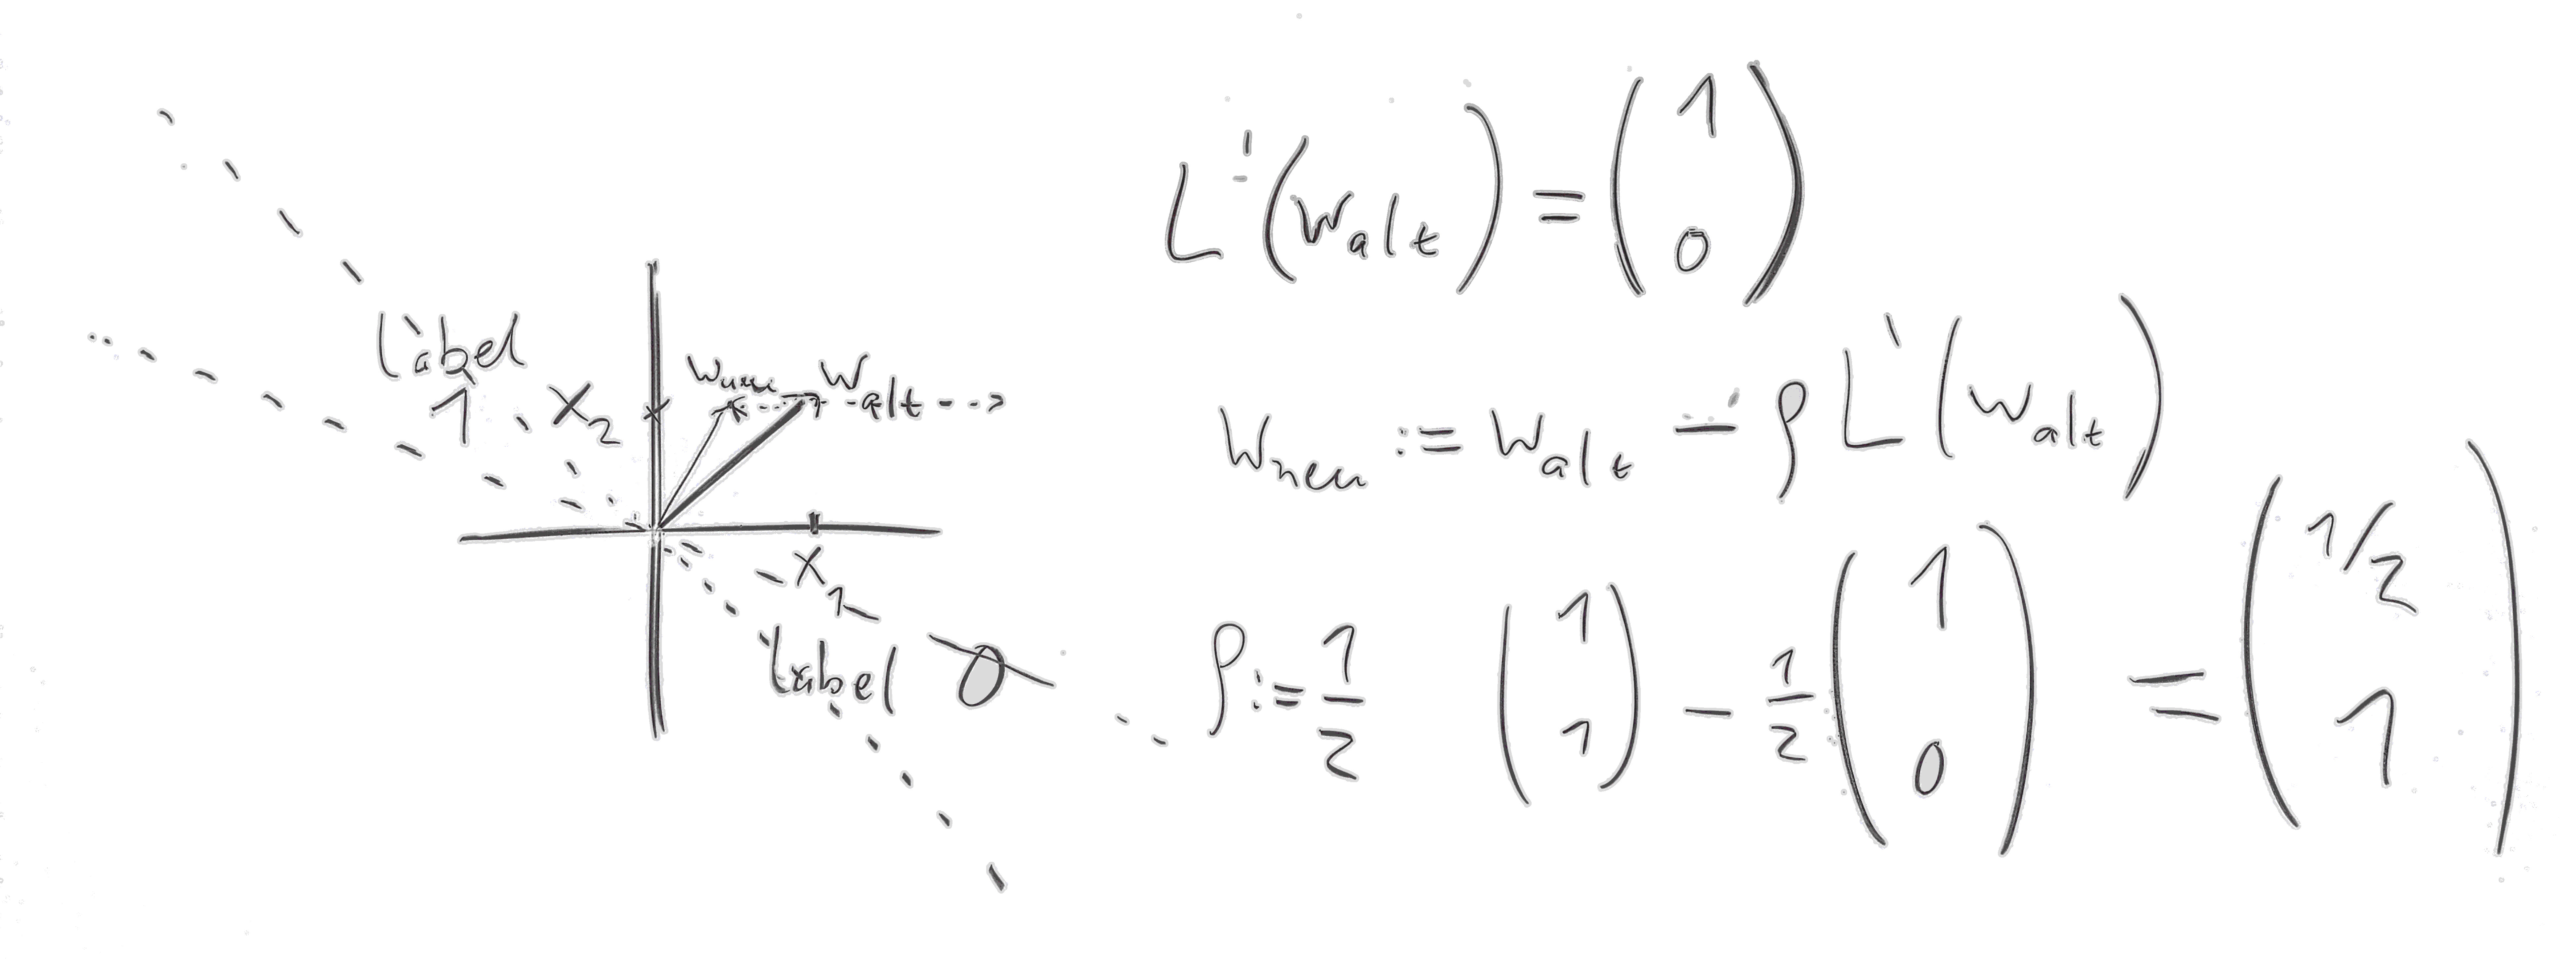
\includegraphics[width=0.62\textwidth]{vl05-tafelbild-gradientenabstieg.jpg}
  \end{center}

  \note{Das ist das Tafelbild aus 2025, hier als Foto. Wer selbst an die Tafel geht,
    kann die Folie überspringen -- dann aber dieselben Zahlen verwenden wie auf den
    Folien, es sollen keine neuen Zahlen an der Tafel stehen.
    \textbf{Hier die Klammer aufmachen:} „Wo steckt in diesem Verfahren eigentlich der
    Zufall?“ -- Frage stellen, Antworten sammeln, \emph{offen lassen}. Auflösung erst
    nach dem Take-Home-Slide.}
\end{frame}

\begin{frame}
  \frametitle{Die Lernrate}

  \begin{columns}[c]
    \begin{column}{0.5\textwidth}
      \Large
      zu klein: ewig unterwegs\\[10pt]
      zu groß: über das Tal hinweg
    \end{column}
    \begin{column}{0.46\textwidth}
      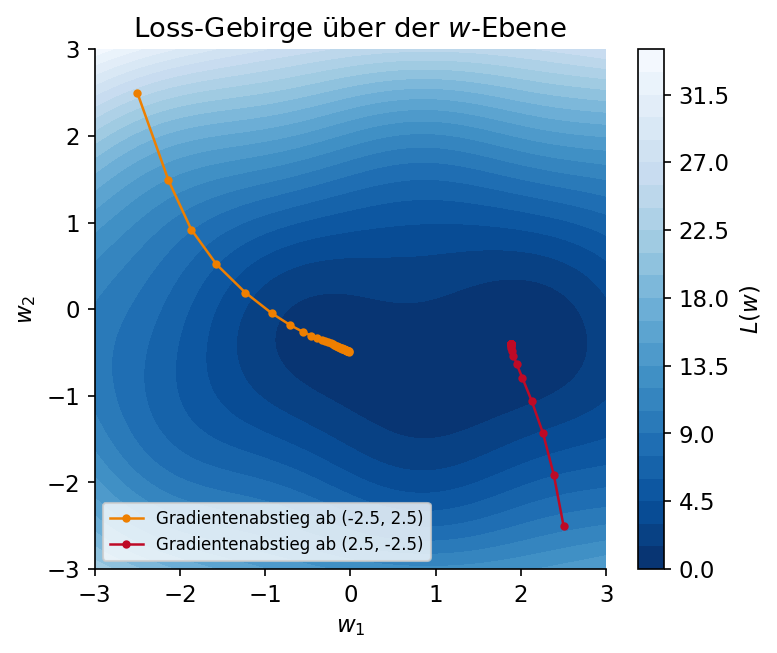
\includegraphics[width=\textwidth]{vl05-loss-landscape.png}
    \end{column}
  \end{columns}

  \note{Loss-Landschaften echter Netze sind nicht konvex, haben viele lokale Minima,
    Sattelpunkte und Plateaus -- und trotzdem funktioniert das Verfahren erstaunlich gut.
    Bild nach Li et al., \emph{Visualizing the loss landscape of neural nets} (2017).}
\end{frame}

\begin{frame}
  \frametitle{Ausprobieren: losslandscape.com/explorer}

  \begin{center}
    \Large Drei Lernraten:\\[12pt]
    \normalsize
    zu klein -- bleibt im ersten Hang\\[6pt]
    mittel -- findet ins Tal\\[6pt]
    zu groß -- springt zwischen den Wänden
  \end{center}

  \note{\textbf{Browser-Block, gut zehn Minuten.} Den Pfad selbst starten lassen.
    Was man mitnimmt: Man kennt die Landschaft im echten Training \emph{nicht}, man sieht
    nur den Loss-Wert. Der Loss steigt auch mal an, ohne dass etwas kaputt ist. Steigt er
    dauerhaft oder wird \texttt{nan}, ist die Lernrate zu groß. In der Praxis fängt man
    groß an und wird kleiner.
    2025 kamen aus dem Hörsaal genau die richtigen Vorschläge: Loss beobachten, bei einem
    Ausreißer neu initialisieren, Lernrate anpassen.}
\end{frame}

\begin{frame}
  \frametitle{Zurück zum Perzeptron}

  \begin{center}
    \Large
    $L_{\text{Perc}}(w) = \sum_i \max\bigl(0, -y_i \langle w, x_i\rangle\bigr)$\\[14pt]
    $L'_{\text{Perc}}(w) = \sum_{i \text{ falsch}} -y_i x_i$
  \end{center}

  \bigskip
  \begin{center}
    \normalsize Für $N = 1$: \quad $w_{\text{neu}} = w_{\text{alt}} \pm \rho\,x$
  \end{center}

  \note{Der „harte“ Perceptron Loss mit \texttt{sign} hätte fast überall Gradient null --
    deshalb die weiche Variante ohne \texttt{sign}: proportional dazu, \emph{wie weit} auf
    der falschen Seite der Punkt liegt. Die schwache Ableitung war eine Übungsaufgabe.
    Und damit ist die Perzeptronregel genau ein Gradientenschritt.
    \emph{Rosenblatt hat 1958 stochastischen Gradientenabstieg gemacht, ohne es so zu
    nennen.} Das ist die schönste Pointe der Sitzung.}
\end{frame}

\begin{frame}
  \frametitle{Und die logistische Regression?}

  \begin{center}
    \Huge $\dfrac{dL}{dz} = p - y$
  \end{center}

  \bigskip
  \begin{center}
    \normalsize Alle Logarithmen und Sigmoide heben sich weg.
  \end{center}

  \note{Die Rechnung an der Tafel: $L(z) = -y\ln\sigma(z) - (1-y)\ln(1-\sigma(z))$,
    mit $\sigma' = \sigma(1-\sigma)$ und Kettenregel bleibt $p - y$ übrig.
    Übrig bleibt der \emph{Vorhersagefehler} -- und mit $\partial z/\partial w = x$ ist
    der Gradient $(p-y)x$. Also dieselbe Gestalt wie die Perzeptronregel.
    Das ist ein Ergebnis, das man sich merkt: Bei Sigmoid plus BCE ist der Gradient
    einfach „Vorhersage minus Wahrheit“.}
\end{frame}

\begin{frame}
  \frametitle{Drei Loss-Funktionen}

  \begin{center}
    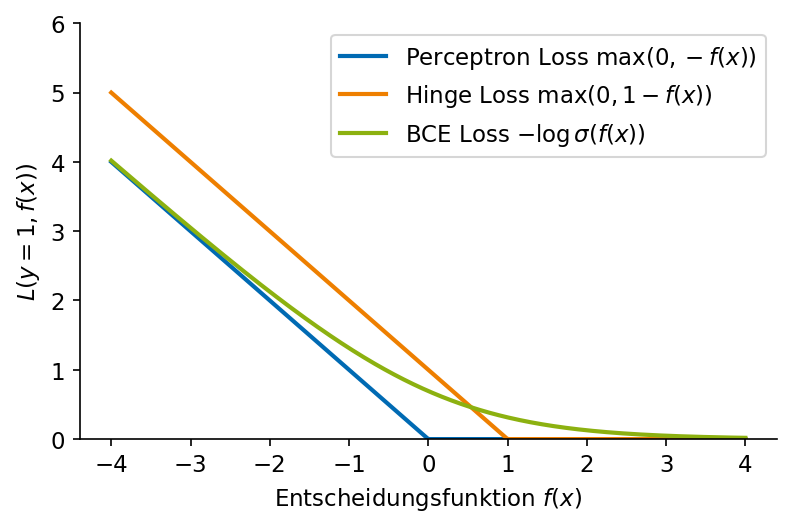
\includegraphics[width=0.58\textwidth]{vl05-loss-curves.png}
  \end{center}

  \note{Für ein Sample mit $y = 1$, aufgetragen gegen $f(x) = \langle w,x\rangle$:
    Perceptron Loss ist null, sobald $f(x) > 0$. Hinge Loss verlangt einen
    Sicherheitsabstand, erst ab $f(x) \ge 1$ null -- das ist der Loss der Support Vector
    Machine. BCE ist glatt und wird nie exakt null, bestraft also auch richtig
    klassifizierte Samples nahe der Grenze noch ein bisschen.}
\end{frame}

\begin{frame}
  \frametitle{Warum man Features skaliert}

  \begin{center}
    \Large
    Körpergröße in Metern \quad gegen \quad Einkommen in Euro\\[16pt]
    \normalsize Gradientenkomponente tausendmal größer,\\
    Krümmung eine Million mal größer.
  \end{center}

  \bigskip
  \begin{center}
    Das Tal ist eine lange, schmale Schlucht.
  \end{center}

  \note{Eine Lernrate, die in der einen Richtung vernünftig vorankommt, springt in der
    anderen heraus. Ausweg: alle Features auf Mittelwert 0 und Standardabweichung 1
    (\texttt{StandardScaler}) -- und das Testset mit den Werten des \emph{Trainingssets}
    skalieren.
    Dieselbe Idee \emph{innerhalb} des Netzes heißt Batch bzw. Layer Normalization; dass
    Adam die Lernrate pro Parameter anpasst, hat denselben Grund. Kommt später.}
\end{frame}

\begin{frame}
  \frametitle{Take-Home}

  \begin{center}
    \Large
    $y_{\text{pred}} = \tau(\langle w, x\rangle)$\\[16pt]
    $w_{\text{neu}} = w_{\text{alt}} - \rho\,L'(w_{\text{alt}})$
  \end{center}

  \bigskip
  \begin{center}
    \normalsize $\tau = \sigma$ und $L = L_{\text{BCE}}$: logistische Regression.
  \end{center}

  \note{Ein Neuron ist Aktivierungsfunktion plus Gewichtsvektor. Training ist immer
    dieselbe Regel; was dabei herauskommt, hängt nur an der Wahl der Loss-Funktion.
    In echt hat man die Augen verbunden, kennt die Landschaft nicht und muss die Lernrate
    ausprobieren.}
\end{frame}

\begin{frame}
  \frametitle{Wo steckt der Zufall?}

  \begin{center}
    \Large
    im Startvektor\\[10pt]
    in den Daten (als Stichprobe modelliert)\\[10pt]
    in der Reihenfolge der Samples
  \end{center}

  \bigskip
  \begin{center}
    \normalsize Deshalb: \emph{stochastischer} Gradientenabstieg.
  \end{center}

  \note{\textbf{Jetzt die Klammer schließen}, die beim Tafelbeispiel aufgemacht wurde.
    Begriffe sauber trennen: \emph{Gradientenabstieg} (Batch) wertet den ganzen Datensatz
    aus; \emph{SGD} schätzt den Gradienten aus einem Teildatensatz, meist einem einzelnen
    Sample. Die Schätzung ist verrauscht, aber im Mittel korrekt -- und man kommt viel
    häufiger zu einem Update.
    Eine Epoche ist ein Durchlauf durch den ganzen Datensatz.}
\end{frame}

\begin{frame}
  \frametitle{Bis nächste Woche}

  \begin{itemize}\setlength{\itemsep}{8pt}
  \item Im \emph{TensorFlow Playground} die sechs Gewichte von Hand so setzen, dass XOR gelöst wird
  \item Mit dem \emph{Loss Landscape Explorer} spielen
  \end{itemize}

  \bigskip
  \begin{center}
    Nächste Woche: Backpropagation -- und danach verstehen Sie den Playground.
  \end{center}

  \note{Beides ist keine Abgabe, sondern Spielaufgabe -- aber das Ziel für nächste Woche
    ist ausdrücklich, den Playground lesen zu können.
    Auf dem Übungsblatt: Ableitung des Sigmoids mit der Quotientenregel, Softmax für $K = 2$,
    Kreuzentropie und Kullback-Leibler-Divergenz.}
\end{frame}

\end{document}

%%% Local Variables:
%%% mode: latex
%%% TeX-master: t
%%% End:
